\newcommand{\xbold}{{\bf x}}
\newcommand{\ibold}{{\bf i}}
\newcommand{\jbold}{{\bf j}}
\newcommand{\kbold}{{\bf k}}
\newcommand{\ebis}{{\tt EBIndexSpace}}
\newcommand{\baseif}{{\tt BaseIF}}
\newcommand{\sphereif}{{\tt SphereIF}}
\newcommand{\transformif}{{\tt TransformIF}}
\newcommand{\latheif}{{\tt LatheIF}}
\newcommand{\unionif}{{\tt UnionIF}}
\newcommand{\intersectionif}{{\tt IntersectionIF}}
\newcommand{\geom}{{\tt GeometryShop}}
\newcommand{\parm}{{\tt ParmParse}}

\section{Overview of Embedded Boundary Description}
\label{sec:EB:EBOverview}

For computations with complex geometries, $\tt{AMReX}$ provides data
structures and iterators for performing Cartesian grid, embedded
boundary (EB) calculations.    In this description, the surface of the
geometry cuts the Cartesian cells.   See figure \ref{fig::ebexample}
for an illustration.    Because this is a relatively simple grid
generation technique, grids can be generated quickly and robustly.
This description can produces arbitrarily small computational volumes,
however.    This can increase the complexity of embedded boundary
algorithms.   This is explained more below.
In this description,
geometry is represented by volumes ($V = \kappa h^d$) and apertures 
($A= \alpha h^{d-1}$).   See figure \ref{fig::volume}
for an illustration.     

\subsection{Finite Volume Discretizations}
Cartesian grids with embedded boundaries are 
useful to describe volume-of-fluid representations of irregular
boundaries.   
Consider a system of hyperbolic equations for a conserved quantity $U$
with fluxes $F$:
\begin{equation}
\frac{\partial U}{\partial t} + \nabla \cdot F = 0.
\label{eqn::hypsys}
\end{equation}
A conservative, finite volume discretization starts with
the divergence theorm
$$
\int_V \nabla \cdot F dV = \int_{\partial V} F \cdot n dA.
$$
In an embedded boundary cell, the divergence is discretized  (as
$D^c(F)$) as follows
\begin{equation}
D^c(F) = \frac{1}{\kappa h} \left( \sum^D_{d = 1}
  (F_{d, hi}A_{d,hi} - F_{d, lo}A_{d,lo})  + F^{EB} A^{EB} \right).
\label{eqn::ebdiv}
\end{equation}
See figure \ref{fig::eb_fluxes} for an illustration.  For a second
order discretization of the divergence, fluxes must be centered at the
centroids of the faces.  
The only geometric information required for second order embedded
boundary algorithms are:
\begin{itemize}
\item
Volume fractions
\item
Area fractions
\item 
Centers of volume, area.
\end{itemize}

\subsection{Small Cells And Hyperbolic Stability}

A naive time discretization of \ref{eqn::hypsys}
using \ref{eqn::ebdiv},
$$
U^{n+1} = U^{n} - \delta t D^c(F)
$$
would have a time step constraint $\dt < h \kappa^{1/D}/V_m$,  that
goes to zero as the size of the 
smallest volume  fraction $\kappa$ in the calculation.  Since these volume fractions can
be arbitrarily small, this is an unacceptable constraint.  One way to remedy
this is to create  non-conservative approximation to the divergence
$D^{nc}$, which at a cell $\ibold$, an average of the conservative divergences in the
$N_\ibold$, the neighborhood of $\ibold$.
$$
D^{nc}(F)_\ibold = \frac{\sum_{\jbold \in N_\ibold}\kappa_\jbold D(F)_\jbold}{\sum_{\jbold \in N_\ibold}\kappa_\jbold}
$$
We then update the solution using a hybrid divergence $D^H(F) =
\kappa D^c(F) + (1-\kappa)D^{nc}$:
$$
U^{n+1,*} = U^n - \delta t D^H(F)
$$
To preserve conservation, we calculate $\delta M$, how much mass was gained or
lost due to not using $D^c$ directly
$$
\delta M_\ibold = \kappa (1-\kappa)(D^c(F)_\ibold - D^{nc}(F)_\ibold)
$$
We then redistribute this extra mass to neighbors.   The mass is
broken up into pieces, one for each neighbor $\jbold \in N_\ibold$:
$$
\delta M_\ibold = \sum_{\jbold \in N_\ibold} \delta M_{\jbold, \ibold}.
$$
A common weighting scheme is  
mass weighting, where higher density cells get more of the
redistribution mass.    If $\rho$ is the mass density, this takes the
form
\begin{equation}
\delta M_{\jbold, \ibold} =  \frac{\delta M_\ibold \kappa_\jbold
  \rho_\jbold}{\sum_{\kbold \in N_\ibold} \kappa_\kbold \rho_\kbold}
\label{eqn::massweight}
\end{equation}
The solution in the neighborhood is updated using this redistribution
mass, for all $\jbold \in N_\ibold$,
$$
U^{n+1}_\jbold = U^{n+1,*}_\jbold + \frac{\delta M_{\jbold,\ibold}}{\kappa_\jbold}.
$$
If one is using the mass weighting scheme (\ref{eqn::massweight}),
this comes out to be
$$
U^{n+1}_\jbold = U^{n+1,*}_\jbold + 
 \frac{\delta M_\ibold
  \rho_\jbold}{\sum_{\kbold \in N_\ibold} \kappa_\kbold \rho_\kbold}.
$$
Note that we no longer divide by the volume fraction.
See  figure \ref{fig::redistribution} for an illustration of a
redistribution neighborhood.   Typically, one uses as a neighborhood
every cell that can be reached via a  monotonic path of unit length.

\begin{figure}[p]
  \centering
  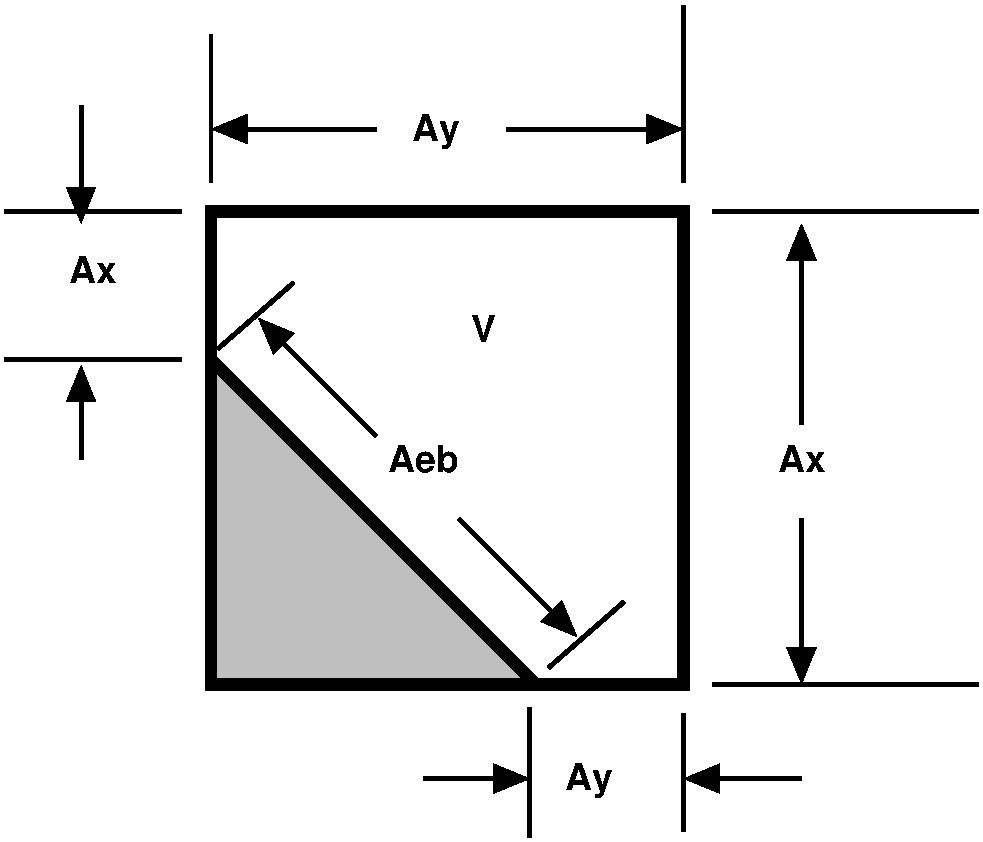
\includegraphics[width=0.5\textwidth]{./EB/areas_and_volumes.pdf}
\caption{\label{fig::volume}Embedded boundary cell. The grey area represents 
the region excluded from the solution.   The areas (labelled with A) are the uncovered
regions of the cell faces.  The volume (labelled V) is the uncovered
region of the interior.}
\end{figure}


\begin{figure}[p]
  \centering
  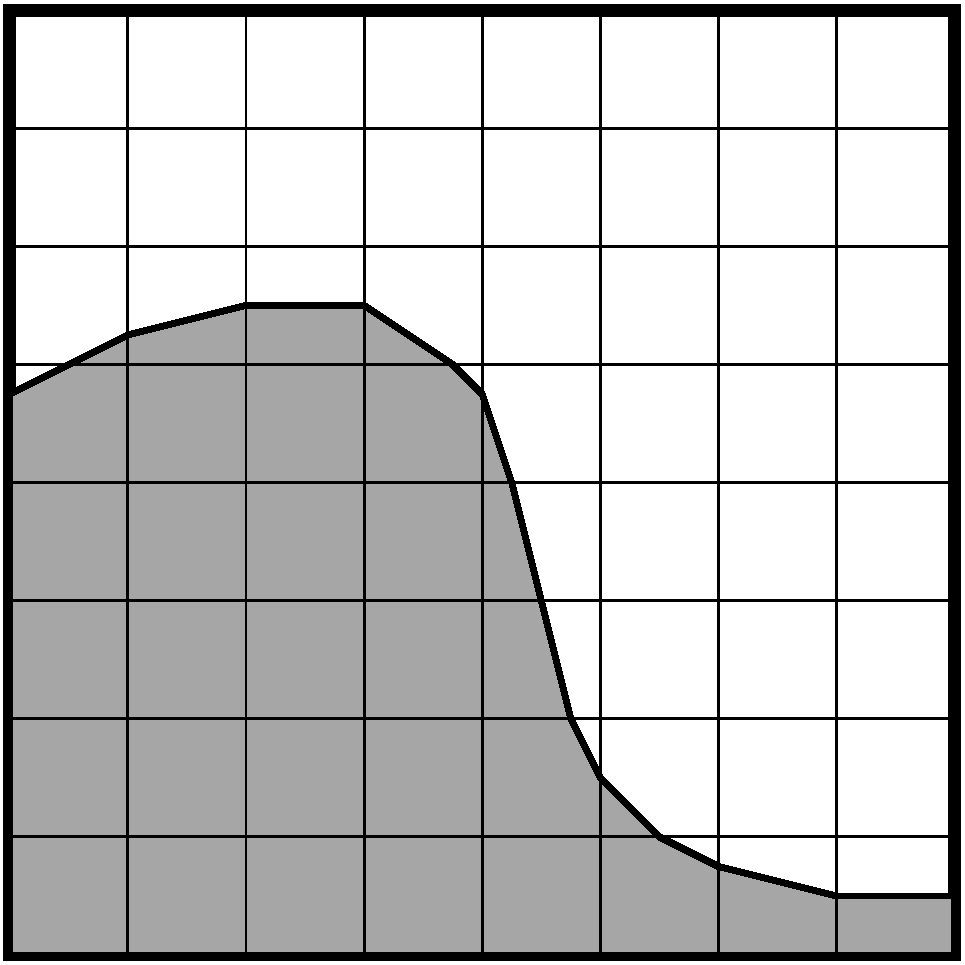
\includegraphics[width=0.5\textwidth]{./EB/EB_example.pdf}
\caption{\label{fig::ebexample}Embedded boundary example.   We cut the
  Cartesian grid with the surface of the geometry.  The parts covered
  by the geometry (the shaded region) are excluded from the domain.}
\end{figure}

\begin{figure}[p]
  \centering
  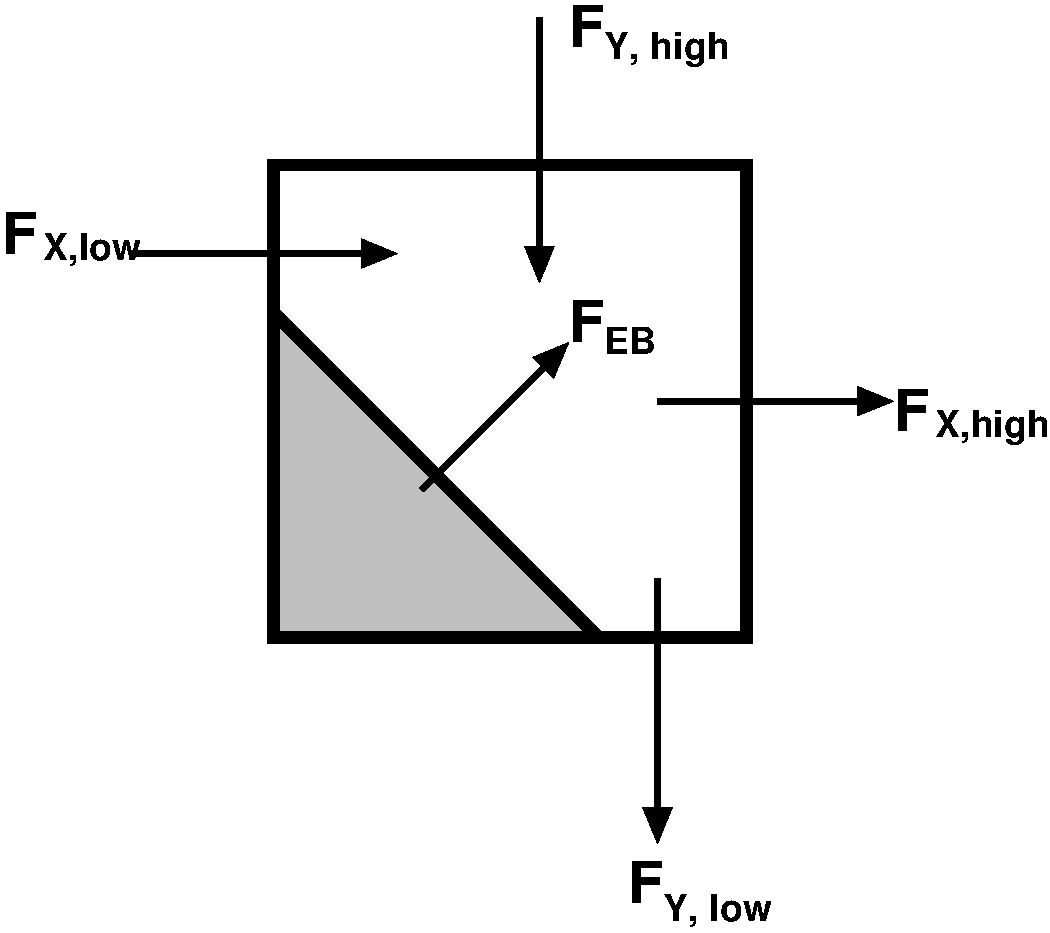
\includegraphics[width=0.5\textwidth]{./EB/eb_fluxes.pdf}
\caption{\label{fig::eb_fluxes}Embedded boundary example.   We cut the
  Cartesian grid with the surface of the geometry.  The parts covered
  by the geometry (the shaded region) are excluded from the domain.}
\end{figure}

\begin{figure}[p]
  \centering
  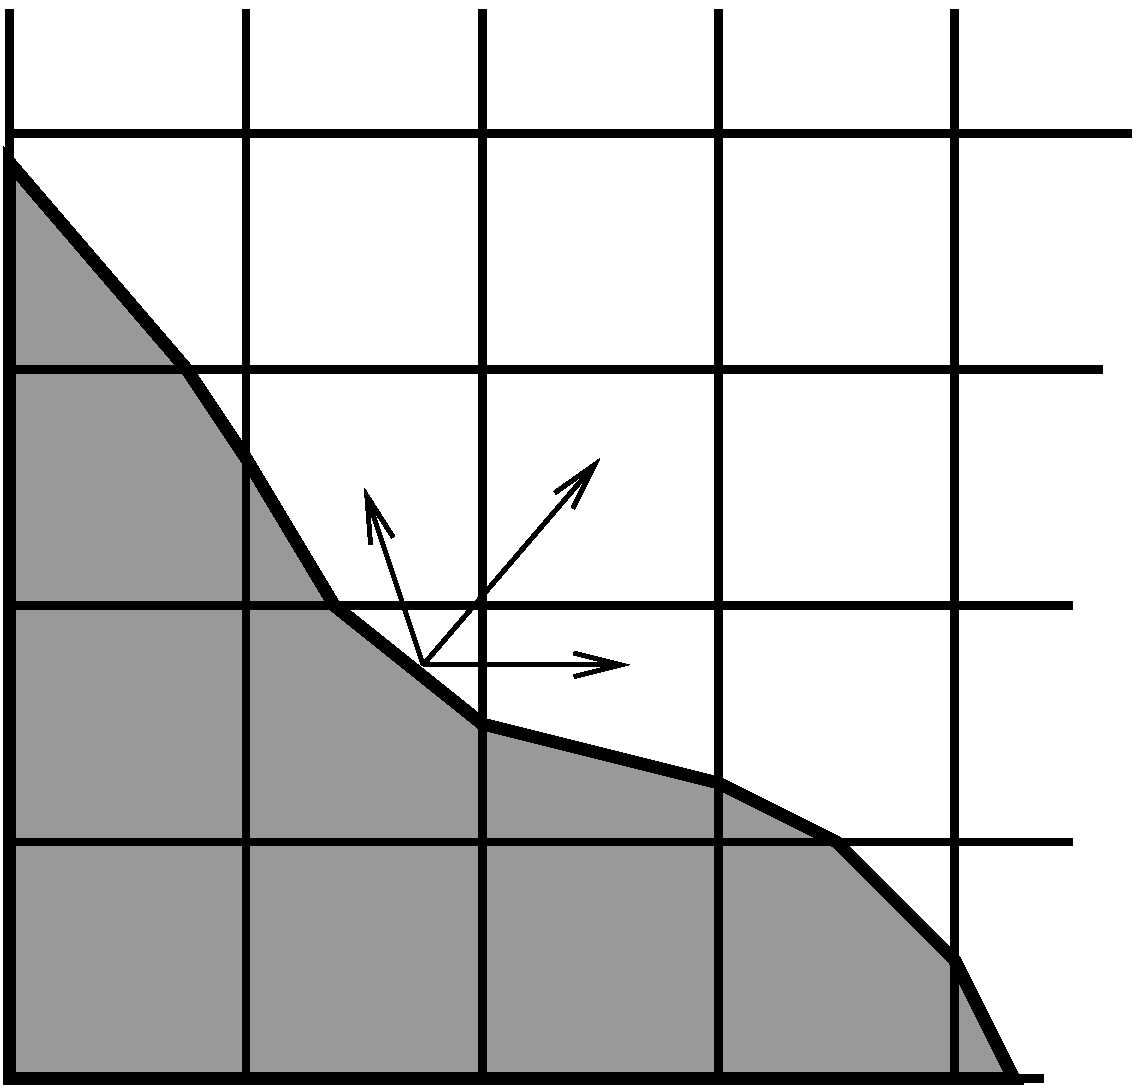
\includegraphics[width=0.5\textwidth]{./EB/redist.pdf}
\caption{\label{fig::redistribution}
Redistribution illustration.  Excess mass due to using a hybrid
divergence $D^H$ instead of the conservative divergence $D^C$ is
distributed among neighbors.}
\end{figure}

\section{Initializing \ebis, the Geometric Database}
\label{sec:EB:ebinit}

This geometric information, along with its associated connectivity
graph is stored in a distributed database class \ebis which must be
initialized at the start of the calculation.    The procedure for this
goes as follows.   To initialize this database, one follows these steps:
\begin{itemize}
\item Define an implicit function which describes the surface 
      and use it define a \geom object (see \S
      \ref{sec:EB:geometryshop}).
\item Call $\tt{EBIndexSpace::define}$ with the \geom object.   This
  will fill the database of graph and moment data.   It is important
  to define this using the finest resolution of domain that will be
  used in the calculation.   Coarser information is generated
  automatically by \ebis by graph coarsening.
\end{itemize}
As an illustration, here is how one would define the \ebis where the
geometry is described as the complement of a sphere of radius 0.1
centered inside a unit cube where the maxium resolution is $1024^3$.
The classes involved are described in \S \ref{sec:EB:geometryshop}.

\begin{lstlisting}[language=cpp]

  int nx = 1024;
  Box domain(IntVect::Zero, (nx-1)*IntVect::Unit);
  Real dx = 1.0/nx;
  Real radius = 0.1;
  Real center = 0.5*RealVect::Unit;
  bool insideRegular = false;
  //this is the implicit function
  SphereIF sphere(radius, center, insideRegular);

  //this is worker object that creates geometric information given an IF
  GeometryShop workshop(sideImpMultisphere)

  //this is the global, distributed database being initialized
  EBIndexSpace*  ebis = AMReX_EBIS::instance()
  ebis->define(domain, RealVect::Zero, dx, workshop);

\end{lstlisting}

%%After this initialization is complete, any part of the calculation can
%%access the data via $\tt{EBIndexSpace::fillEBISLayout}$.

\subsection{GeometryShop and Implicit Functions}
\label{sec:EB:geometryshop}

One of the greatest advantages of EB technology is that grid
generation is robust and fast and can be done to any accuracy
The foundation class that AMReX uses for
geometry generation is called \geom.  Given an implicit
function $I$  \geom interprets the surface upon which $I(\xbold) = 0$
as the surface with which to cut the grid cells.   \geom interprets
the positive regions of the implicit function ($\xbold: I(\xbold) > 0$)
as covered by the geometry  negative regions ($\xbold: I(\xbold) < 0$) 
as part of  the solution domain.  For example, if one defines her
implicit function $S$ as
$$
S(\xbold) = x^2 + y^2 + z^2 - R^2,
$$
the solution domain would be the interior of a sphere of radius $R$.
Reverse the sign of $S$ and the solution domain would be the exterior
of the sphere.   

To define a geometry shop, one
needs to send it a \baseif, which describes an implict function. 

\begin{lstlisting}[language=cpp]
    GeometryShop(const BaseIF& a_localGeom)
\end{lstlisting}

The implicit function must be able to return the value of the function at any
point in space.

\begin{lstlisting}[language=cpp]
    /// Return the value of the function at a_point.  
    virtual Real value(const RealVect& a_point) const = 0;
\end{lstlisting}

\subsection{Simple Implicit Function Example, Sphere}

If one wants to define a geometry
as a domain with  a sphere cut out of it, one uses the \sphereif
class, the functions of which are shown below.

\begin{lstlisting}[language=cpp]
    SphereIF::
    SphereIF(const Real&     a_radius,
             const RealVect& a_center,
             const bool&     a_inside)
    {
     m_radius  = a_radius;
     m_radius2 = m_radius*m_radius;
     m_inside  = a_inside;
     m_center  = a_center;
    }

  Real
  SphereIF::
  value(const RealVect& a_point) const
  {
    RealVect dist = a_point - m_center;
    Real distance2 = dist.radSquared();
    Real retval = distance2 - m_radius2;
    // Change the sign to change inside to outside
    if (!m_inside)
      {
        retval = -retval;
      }

    return retval;
  }
  BaseIF* 
  SphereIF::
  newImplicitFunction() const
  {
    SphereIF* spherePtr = new SphereIF(m_radius,
                                       m_center,
                                       m_inside);

    return static_cast<BaseIF*>(spherePtr);
  }
\end{lstlisting}

\subsection{Implicit Function Transformation Tools}

One can get by with very simple implicit functions such as sphere and
plane because one can create more complicated geometries by
composition of simple implicit functions.    AMReX contains the
following classes which are used compose implicit functions.
\begin{itemize}
\item $\tt{TransformIF}$    allows for translations and rotations of an implicit function.
\item $\tt{UnionIF}$        produces the union of two implicit functions.  
\item $\tt{IntersectionIF}$ produces the intersection of two implicit functions.
\item $\tt{LatheIF}$        creates a 3D implicit function as the surface of
  revolution of a 2D implicit function.

\end{itemize}
\subsection{Geometric example 1 -- Multi-sphere}
Here is an example that uses many of these tools.  This example
creates a geometry with multiple spheres cut out.

\begin{lstlisting}[language=cpp]

//say you have a bunch of radii and centers of spheres
/* fill these in however you like */
vector<Real>     radius(numSpheres);
vector<RealVect> center(numSpheres);
...
//create an implicit function for each sphere
vector<BaseIF*>  spheres(numSpheres);

for(int isphere = 0; isphere < numSpheres; isphere++)
{
  //create each sphere at the origin and translate
  SphereIF sphereAtZero(radius[isphere], RealVect::Zero, false);
  TransformIF* movedSphere = new TransformIF(sphereAtZero);
  movedSphere->translate(center[isphere]);
  spheres[isphere] = static_cast<BaseIF*>(movedSphere);
}
//create an implicit function that is the intersection of all the spheres
IntersectionIF impMultisphere(spheres);
//we want the fluid to be the complement (the space outside the sphere
ComplementIF sideImpMultisphere(impMultisphere, false);
//create the geometryshop
GeometryShop workshop(sideImpMultisphere)
\end{lstlisting}

\subsection{Geometric example 2 -- Surface of revolution}

Here is an example that creates a geometric construction using a
surface of revolution of a set of polygons.   This particular example
only makes sense in three dimensions.

\begin{lstlisting}[language=cpp]

/// define EBIndexSpace from the surface of revolution of a set of polygons
void
defineGeometry(const Real& fine_dx, const  Box& finest_domain, int max_grid_size)
{
  amrex::Print() << "creating geometry from polygon surfaces of revolution" << endl;

  // These  the polygons that get built around the z axis
  Array<Array<RealVect> > polygons;
  //....fill the polygons any way you like//

  // Make the Array of (convex) polygons (Arrays of points) into a union
  // of convex polygons, each made from the intersection of a set of half
  // planes/spaces - all represented by implicit functions.

  // A list of all the polygons as implicit functions
  Array<BaseIF*> polytopes;
  polytopes.resize(0);
  int numPolys = polygons.size();
  // Process each polygon
  for (int p = 0; p < numPolys; p++)
  {
    // All the half planes/spaces used to make a polygon
    Array<BaseIF*> planes;
    planes.resize(0);

    // Get the current polygon (as a Array of points)
    const Array<RealVect>& polygon = polygons[p];

    // Get the number of points in the polygon
    int numPts = polygon.size();

    // Process each pair of points
    for (int n = 0; n < numPts; n++)
    {
      // The normal and point is space used to specify each half plane/space
      RealVect normal(RealVect::Zero);
      RealVect point;

      // Set the normal remembering that the last point connects to the first
      // point.
      normal[0] = -(polygon[(n+1) % numPts][1] - polygon[n][1]);
      normal[1] =  (polygon[(n+1) % numPts][0] - polygon[n][0]);

      point = polygon[n];

      // Generate the appropriate half plane/space (as an implicit function)
      PlaneIF* plane;
      plane = new PlaneIF(normal,point,true);

      // Save the result
      planes.push_back(plane);
    }

    // Intersect all the half planes/spaces to create an implicit function
    // that represents the polygon
    IntersectionIF* polygonIF = new IntersectionIF(planes);

    polytopes.push_back(polygonIF);
  }

  //this makes the cross section the union of all the polgons (around
  //z-axis, recall)
  UnionIF crossSection(polytopes);
            
  // In 3D rotate about the z-axis 
  LatheIF lathe(crossSection, false);

  //we are starting around the z axis so we need to translate
  //over to the center of the x-y plane
            
  RealVect translation;
  for(int idir = 0; idir < SpaceDim; idir++)
  {
    translation[idir] = 0.5*finest_domain.size()[idir]*fine_dx;
  }
  translation[2] = 0;
  TransformIF implicit(lathe);
  implicit.translate(translation);

  //create a workshop from translated surface of revolution
  GeometryShop gshop(implicit, false);
  //define th geometric database
  AMReX_EBIS::instance()->define(finest_domain, RealVect::Zero,
                                 fine_dx, gshop, max_grid_size);
}

\end{lstlisting}

\section{$\tt{EBFarrayBox}$}

The fundamental data structure for embedded boundary calculations is 
$\tt{EBFArrayBox}$, a class is an a $\tt{FArrayBox}$ with two extra
data members.
\begin{itemize}
\item $\tt{EBFArrayBox::getEBISBox}$ returns an $\tt{EBISBox}$, a data
  structure that contains the graph and geometric information for a
  particular box.
\item $\tt{EBFArrayBox::getEBCellFlagFab}$  is a
  $\tt{BaseFab<EBCellFlag>}$, where $\tt{EBCellFlag}$ is a class which
  is a very compact class that specify connectivity information
  (number of volumes in the cell, which cells are connected to my
  cell...) for a particular cell.
\end{itemize}
If one compiles with $\tt{AMREX\_USE\_EB = TRUE}$, the state data that
${\tt Amr}$ generates is already of type $\tt{EBFArrayBox}$ under the
hood and one can access the functions via cast.   The
$\tt{EBCellFlagFab}$ can be used to choose whether it is necessary to call an
EB-specfic routine. $\tt{EBCellFlagFab}$  can be sent also be sent to Fortran to 
enable EB-specific logic.   

\subsection{Example}
The example below is a simplified version
of one of the routines in $\tt{Tutorial/EB/CNS}$.   Note  that  it
carefully calls the more complicated EB fortran routine if the
particular tile has cut cells.

\begin{lstlisting}[language=cpp]
void
CNS::compute_dSdt (const MultiFab& S, MultiFab& dSdt, Real dt,
                   EBFluxRegister* fr_as_crse, EBFluxRegister* fr_as_fine)
{
    BL_PROFILE("CNS::compute_dSdt()");

    const Real* dx = geom.CellSize();
    const int ncomp = dSdt.nComp();

#ifdef _OPENMP
#pragma omp parallel
#endif
     {
        //fluxes for the advance
        std::array<FArrayBox,AMREX_SPACEDIM> flux;

        for (MFIter mfi(S, MFItInfo().EnableTiling(hydro_tile_size).SetDynamic(true));
                        mfi.isValid(); ++mfi)
        {
            //this tile is the subset of the box over which we are computing
            const Box& bx = mfi.tilebox();

            //because we have compiled with AMREX_USE=EB_TRUE, the
            //MultiFab holds EBFArrayBox(es) so we can do this cast
            const EBFArrayBox& sfab = dynamic_cast<EBFArrayBox
            const&>(S[mfi]);
            
            //here we are getting the collection of flags so we know
            //kind of grid this is and if it is an EB grid, we have
            //the connectivity info
            const EBCellFlafgFab & flag = sfab.getEBCellFlagFab();

            if (flag.getType(bx) == FabType::covered) 
            {
              //this tile is covered so there are no meaningful data here
                dSdt[mfi].setVal(0.0, bx, 0, ncomp);
            } 
            else 
            {
              //create the flux holders for this tile
              for (int idim=0; idim < AMREX_SPACEDIM; ++idim) 
              {
                flux[idim].resize(amrex::surroundingNodes(bx,idim),ncomp);
              }

              if (flag.getType(amrex::grow(bx,1)) == FabType::regular)
              {
                //this tile has no cut cells so we can just proceed
                //with a (cheaper) non-eb call

                cns_compute_dudt(BL_TO_FORTRAN_BOX(bx),
                BL_TO_FORTRAN_ANYD(dSdt[mfi]),
                BL_TO_FORTRAN_ANYD(S[mfi]),
                BL_TO_FORTRAN_ANYD(flux[0]),
                BL_TO_FORTRAN_ANYD(flux[1]),
                BL_TO_FORTRAN_ANYD(flux[2]),
                dx, &dt);

              }
              else
              {
                //this tile has cut cells so we have to send into Fortran
                //EBCellFlagFAB as well as lots of geometric
                //information
                //the areafrac and facecent objects are member data
                //filled using EBISBox
                cns_eb_compute_dudt(BL_TO_FORTRAN_BOX(bx),
                BL_TO_FORTRAN_ANYD(dSdt[mfi]),
                BL_TO_FORTRAN_ANYD(S[mfi]),
                BL_TO_FORTRAN_ANYD(flux[0]),
                BL_TO_FORTRAN_ANYD(flux[1]),
                BL_TO_FORTRAN_ANYD(flux[2]),
                BL_TO_FORTRAN_ANYD(flag),
                BL_TO_FORTRAN_ANYD(volfrac[mfi]),
                BL_TO_FORTRAN_ANYD(bndrycent[mfi]),
                BL_TO_FORTRAN_ANYD(areafrac[0][mfi]),
                BL_TO_FORTRAN_ANYD(areafrac[1][mfi]),
                BL_TO_FORTRAN_ANYD(areafrac[2][mfi]),
                BL_TO_FORTRAN_ANYD(facecent[0][mfi]),
                BL_TO_FORTRAN_ANYD(facecent[1][mfi]),
                BL_TO_FORTRAN_ANYD(facecent[2][mfi]),
                dx, &dt);
              }
            }
          }
        }

\end{lstlisting}

\subsection{Fortran bits}

Now the Fortran that underlies these two cases is quite different.
For the non-EB case,    the one loop in the function is given by the
familiar-looking example below:
\begin{lstlisting}[language=Fortran]
    do n = 1, ncomp
       do       k = lo(3),hi(3)
          do    j = lo(2),hi(2)
             do i = lo(1),hi(1)
                ut(i,j,k,n) = (fx(i,j,k,n)-fx(i+1,j,k,n)) * dxinv(1) &
                     +        (fy(i,j,k,n)-fy(i,j+1,k,n)) * dxinv(2) &
                     +        (fz(i,j,k,n)-fz(i,j,k+1,n)) * dxinv(3)
             end do
          end do
       end do
    end do
\end{lstlisting}

For the embedded boundary version, the code must is much more
complicated. To avoid instabilities associated with arbitrarily small
cells, the divergence is computed in stages.  For this discussion
$\kappa$ is the volume fraction of a cell.  The stages of the
divergence are given by
\begin{itemize}
\item Compute the $\kappa$-weighted divergence.
\item Compute a nonconservative approximation to the divergence that
  is a local average of the previous object.
\item Update the state with a hybrid divergence.
\item Redistribute  mass to preserve conservation.
\end{itemize}
It is beyond the scope of this document to explain all that.  We
include it only to provide the context that EB stencils can be much
more complex that non-EB ones.   Suffice
it to say that the first step of that process is most closely related
to the code above.    The loop that computes the $\kappa$-weighted
divergence is given below.

\begin{lstlisting}[language=Fortran]
    do n = 1, ncomp

       !
       ! First, we compute conservative divergence on (lo-2,hi+2)
       !
       iwall = 0
       do       k = lo(3)-2, hi(3)+2
          do    j = lo(2)-2, hi(2)+2
             do i = lo(1)-2, hi(1)+2
                divc(i,j,k) = (fluxx(i,j,k,n)-fluxx(i+1,j,k,n))*dxinv(1) &
                     +        (fluxy(i,j,k,n)-fluxy(i,j+1,k,n))*dxinv(2) &
                     +        (fluxz(i,j,k,n)-fluxz(i,j,k+1,n))*dxinv(3)
             end do

             do i = lo(1)-2, hi(1)+2
                if (is_covered_cell(cellflag(i,j,k))) then
                   divc(i,j,k) = 0.d0
                else if (is_single_valued_cell(cellflag(i,j,k))) then

                   call get_neighbor_cells(cellflag(i,j,k),nbr)

                   ! x-direction lo face
                   if (apx(i,j,k).lt.1.d0) then
                      if (centx_y(i,j,k).le.0.d0) then
                         fracy = -centx_y(i,j,k)*nbr(0,-1,0)
                         if(centx_z(i,j,k).le. 0.0d0)then
                            fracz = - centx_z(i,j,k)*nbr(0,0,-1)
                            fxm = (1.d0-fracz)*(     fracy *fluxx(i,j-1,k  ,n)  + &
                                 &             (1.d0-fracy)*fluxx(i,j  ,k  ,n)) + &
                                 &      fracz *(     fracy *fluxx(i,j-1,k-1,n)  + &
                                 &             (1.d0-fracy)*fluxx(i,j  ,k-1,n))
                         else
                            fracz =  centx_z(i,j,k)*nbr(0,0,1)
                            fxm = (1.d0-fracz)*(     fracy *fluxx(i,j-1,k  ,n)  + &
                                 &             (1.d0-fracy)*fluxx(i,j  ,k  ,n)) + &
                                 &      fracz *(     fracy *fluxx(i,j-1,k+1,n)  + &
                                 &             (1.d0-fracy)*fluxx(i,j  ,k+1,n))
                         endif
                      else
                         fracy = centx_y(i,j,k)*nbr(0,1,0)
                         if(centx_z(i,j,k).le. 0.0d0)then
                            fracz = -centx_z(i,j,k)*nbr(0,0,-1)
                            fxm = (1.d0-fracz)*(     fracy *fluxx(i,j+1,k  ,n)  + &
                                 &             (1.d0-fracy)*fluxx(i,j  ,k  ,n)) + &
                                 &      fracz *(     fracy *fluxx(i,j+1,k-1,n)  + &
                                 &             (1.d0-fracy)*fluxx(i,j  ,k-1,n))
                         else
                            fracz = centx_z(i,j,k)*nbr(0,0,1)
                            fxm = (1.d0-fracz)*(     fracy *fluxx(i,j+1,k  ,n)  + &
                                 &             (1.d0-fracy)*fluxx(i,j  ,k  ,n)) + &
                                 &      fracz *(     fracy *fluxx(i,j+1,k+1,n)  + &
                                 &             (1.d0-fracy)*fluxx(i,j  ,k+1,n))
                         endif
                      end if
                   else
                      fxm = fluxx(i,j,k,n)
                   end if

           ![***REDACTED-- THERE ARE SIMILAR TERMS FOR XHI, YLO, YHI, ZLO, ZHI***]

                   iwall = iwall + 1
                   if (n .eq. 1) then
                      call compute_hyp_wallflux(divhyp(:,iwall), i,j,k, q(i,j,k,qrho), &
                           q(i,j,k,qu), q(i,j,k,qv), q(i,j,k,qw), q(i,j,k,qp), &
                           apx(i,j,k), apx(i+1,j,k), &
                           apy(i,j,k), apy(i,j+1,k), &
                           apz(i,j,k), apz(i,j,k+1))
                      call compute_diff_wallflux(divdiff(:,iwall), dxinv, i,j,k, &
                           q, qlo, qhi, &
                           lam, mu, xi, clo, chi, &
                           bcent, blo, bhi, &
                           apx, axlo, axhi, &
                           apy, aylo, ayhi, &
                           apz, azlo, azhi)
                   end if

                   divwn = divhyp(n,iwall) + divdiff(n,iwall)

                   ! we assume dx == dy == dz
                   divc(i,j,k) = -((apx(i+1,j,k)*fxp - apx(i,j,k)*fxm) * dxinv(1) &
                        +          (apy(i,j+1,k)*fyp - apy(i,j,k)*fym) * dxinv(2) &
                        +          (apz(i,j,k+1)*fzp - apz(i,j,k)*fzm) * dxinv(3) &
                        +          divwn * dxinv(1)) / vfrac(i,j,k)
                end if
             end do
          end do
       end do

\end{lstlisting}
This should explain why it is desirable to avoid 
calling the EB-specific routine when possible.
